\documentclass[12pt]{article}

% Layout.
\usepackage[top=1in, bottom=0.75in, left=1in, right=1in, headheight=1in, headsep=6pt]{geometry}

% Fonts.
\usepackage{mathptmx}
\usepackage[scaled=0.86]{helvet}
\renewcommand{\emph}[1]{\textsf{\textbf{#1}}}

% TiKZ.
\usepackage{tikz, pgfplots}
\usetikzlibrary{calc}

% Misc packages.
\usepackage{amsmath,amssymb,latexsym}
\usepackage{graphicx}
\usepackage{array}
\usepackage{xcolor}
\usepackage{multicol}
\usepackage{fancyhdr}
\usepackage{tikz}

\pagestyle{fancy}


% Misc.
\renewcommand{\d}{\displaystyle}
\newcommand{\ds}{\displaystyle}
\def\bc{\begin{center}}
\def\ec{\end{center}}
\def\be{\begin{enumerate}}
\def\ee{\end{enumerate}}

\newcommand{\ans}[1][1in]{\rule{#1}{.5pt}}


\lhead{Math F113X: Quiz 6}

\begin{document}

\ 

%\vspace{.25cm}

\noindent \textbf{Name:} \hrulefill \quad  score:\ans[1cm] \ / 10 \\


There are 10 points possible on this quiz. No aids (book, notes, etc.)
are permitted. You may use a non-programmable calculator.  {\bf Show
all work and supporting calculations for full credit. Explain how you
get your answers.}



\be
\item
\be
\item (3 pts.) For the graph below, apply the {\bf Nearest Neighbor} (NN) Algorithm starting at vertex A to find a low weight Hamiltonian cycle.

\begin{center}
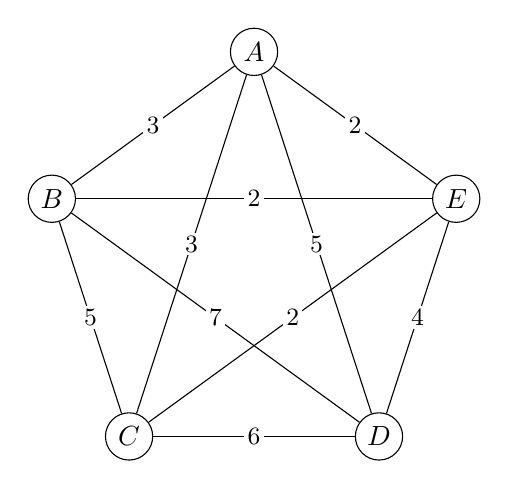
\begin{tikzpicture}[scale = 0.9,
    vertex/.style={circle, draw=black, minimum size=6mm, inner sep=0pt},
    weight/.style={font=\small, fill=white, inner sep=1.2pt}
]
    \def\n{5}
    \def\radius{3cm}
    \foreach \i/\l in {1/A, 2/B, 3/C, 4/D, 5/E} {
        \node[vertex] (v\i) at ({360/\n * (\i - 1) + 90}:\radius) {$\l$};
    }
    % Edges from A
    \draw (v1) -- node[weight] {3} (v2);
    \draw (v1) -- node[weight] {3} (v3);
    \draw (v1) -- node[weight] {5} (v4);
    \draw (v1) -- node[weight] {2} (v5);
    % Edges from B
    \draw (v2) -- node[weight] {5} (v3);
    \draw (v2) -- node[weight] {7} (v4);
    \draw (v2) -- node[weight] {2} (v5);
    % Edges from C
    \draw (v3) -- node[weight] {6} (v4);
    \draw (v3) -- node[weight] {2} (v5);
    % Edges from D
    \draw (v4) -- node[weight] {4} (v5);
\end{tikzpicture}
\end{center}

\noindent
Circuit (List vertices):\underline{\hskip 3.in}

\ 

\noindent
Total weight of circuit:\underline{\hskip 3.in}

\ 

\item (1 pt.) The repeated Nearest Neighbor (RNN) Algorithm is more work than the NN Algorithm. Why is it still worth doing?
\vskip 1.in

\item (3 pts.) Describe one real-world situation for which finding a Hamiltonian Circuit in the graph above would be useful.

Vertices represent \underline{\hskip 3.in}

Edge weights represent \underline{\hskip 3.in}

Reason to find a low weight Hamiltonian Cycle:
\vskip 1.in

%\item Briefly describe what more would need to be done to apply the RNN Algorithm to this graph.
%\vskip 1.in

\ee

\newpage

\item (3 pts.)
Use the {\bf Sorted Edges} Algorithm to find a low total weight Hamiltonian circuit for the graph with edge weights described by the following tables. You may find it helpful to draw your circuit using the labelled vertices.

{\centering
\begin{tabular}{c|ccccc}
 & {A} &{B} & {C} & {D} & {E} \\ 
A & - & 10 & 15 & 20 & 10 \\
B & 10 & - & 35 & 25 & 12 \\
C & 15 & 35 & - & 30 & 5 \\
D & 20 & 25 & 30 & - & 10 \\
E & 10 & 12 & 5 & 10 & - 
\end{tabular}
\hskip .5in
\begin{tabular}{c|c|c}
Edge & Weight &used?\\
 \hline
CE&5\\
AB & 10\\
AE&10\\
DE&10\\
BE&12\\
AC&15\\
AD&20\\
BD&25\\
CD&30\\
BC&35\\
\end{tabular}

\ 


\ 


\  

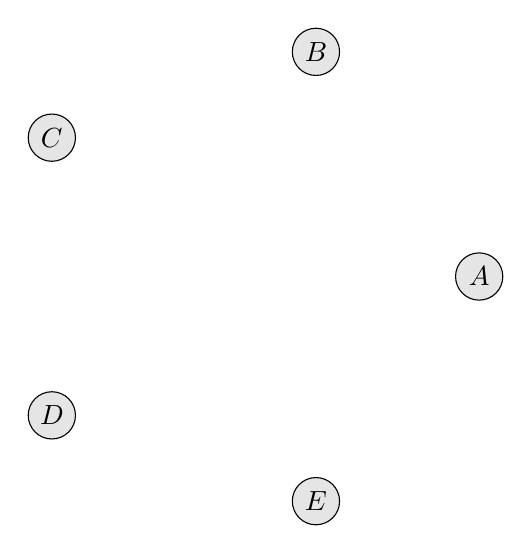
\begin{tikzpicture}[
    % Define a style for the vertices
    vertex/.style={circle, draw=black, fill=gray!20, inner sep=2pt, minimum size=6mm}
]

    % Define the number of vertices and the radius
    \def\n{5}
    \def\radius{3cm}
    % Calculate the angle difference for a regular pentagon (360/5 = 72 degrees)
    \def\angleDiff{72}

    % Place the nodes using a foreach loop and polar coordinates (angle:radius)
    \foreach \i/\label in {0/A, 1/B, 2/C, 3/D, 4/E} {
        \node[vertex] (v\label) at ({\i * \angleDiff}:\radius) {$\label$};
    }

   
    \end{tikzpicture}
\ 


\ 

\ 


}

\noindent
Circuit (List vertices):\underline{\hskip 3.in}

\ 

\noindent
Total weight of circuit:\underline{\hskip 3.in}

\ee

\end{document}
%%% Local Variables:
%%% mode: LaTeX
%%% TeX-master: t
%%% End:
